% =========================================================================
% SciPost LaTeX template
% Version 1a (2016/06/14)
%
% Submissions to SciPost Journals should make use of this template.
%
% INSTRUCTIONS: simply look for the `TODO:' tokens and adapt your file.
%
% - please enable line numbers (package: lineno)
% - you should run LaTeX twice in order for the line numbers to appear
% =========================================================================


% TODO: uncommente ONE of the class declarations below
% If you are submitting a paper to SciPost Physics: uncomment next line
\documentclass{SciPost}
% If you are submitting a paper to SciPost Physics Lecture Notes: uncomment next line
%\documentclass[LectureNotes]{SciPost}
\usepackage{amsmath,amssymb,graphicx,bm,color,mathrsfs,verbatim,epstopdf,dcolumn,cancel}

%%%%%%%%%%%%%%%%%%%%%%%%%%%%%%%%%%%%%%%%%%%%%%%%%%%%%%%%%%%%%%%%

%hyperrefs
\usepackage{hyperref}
\hypersetup{ 
	colorlinks=true,
}


%define path for figs
\usepackage{graphicx}
\usepackage{caption}
\usepackage{subcaption}
% needed for \sout{}
%\usepackage[normalem]{ulem}

%%%%%%%%%%%%%%%%%%%%%%%%%%%%%%%%%%%%%%%%%%%%%%%%%%%%%%%%%%%%%%%%
%%%%%%%%%%%%%%%%%%%% Python code %%%%%%%%%%%%%%%%%%%%%%%%%%%%%%%
%%%%%%%%%%%%%%%%%%%%%%%%%%%%%%%%%%%%%%%%%%%%%%%%%%%%%%%%%%%%%%%%

\usepackage{listings}
% the following lines make sure the pdf code is copy-pastable
\usepackage{textcomp}
\usepackage[space=true]{accsupp}

\newcommand{\pdfactualhex}[3]{\newcommand{#1}{%
		\BeginAccSupp{method=hex,ActualText=#2}#3\EndAccSupp{}}}

\pdfactualhex{\pdfactualdspace}{2020}{\textperiodcentered\textperiodcentered}
\pdfactualhex{\pdfactualsquote}{27}{'}
\pdfactualhex{\pdfactualbtick}{60}{`}

% define colours 
\definecolor{deepblue}{rgb}{0,0,0.8}
\definecolor{deepred}{rgb}{1.0,0,0}
\definecolor{deepgreen}{rgb}{0,0.7,0}
\definecolor{blueviolet}{RGB}{138,43,226}
\definecolor{darkyellow}{RGB}{204,204,0}
\definecolor{codegray}{rgb}{0.6,0.6,0.6}
\definecolor{weborange}{RGB}{255,165,0}
\definecolor{gold}{RGB}{255,205,0}
\definecolor{codegreen}{rgb}{0,0.6,0}
\definecolor{codepurple}{rgb}{0.58,0,0.82}

%\definecolor{backcolour}{rgb}{0.0,0.0,0.0}
\definecolor{backcolour}{rgb}{0.95,0.95,0.92}

\lstdefinestyle{sublime}{
	backgroundcolor=\color{backcolour},   
	commentstyle=\color{deepgreen},
	keywordstyle=\color{deepred},
	numberstyle=\tiny,
	stringstyle=\color{weborange},
	basicstyle=\small\ttfamily, %\footnotesize,
	breakatwhitespace=false,         
	breaklines=true,                 
	captionpos=t,                    
	keepspaces=true,                 
	numbers=left,                    
	numbersep=5pt,                  
	showspaces=false,                
	showstringspaces=false,
	showtabs=false,                  
	tabsize=4,
	columns=flexible,
	emptylines=10000,
	literate={'}{\pdfactualsquote}1{`}{\pdfactualbtick}1{\ \ }{\pdfactualdspace}2,
	inputpath=./anc,
%	inputpath=anc/,
	keywords={lambda,xrange,abs,for,return},
}
\lstset{style=sublime,language=Python}

% change default listings caption title
\renewcommand{\lstlistingname}{QuSpin \emph{Example Code}}% Listing -> q\spin\ Example Code


%%%%%% the following lines put the slashed zero in the code environtmnet listings

\usepackage{marvosym,etoolbox}
% this replaces 0 with \0 in lstings
\lstset{literate={0}{\0}1{0\ }{\0\ }2}

\renewcommand*\ttdefault{txtt}
\usepackage[T1]{fontenc}
\usepackage{graphicx}
% defines \0 as mirro of 0
\newcommand\0{\scalebox{-1}[1]{0}}
% fix for \texttt and \ttfamily
\let\svttfamily\ttfamily
\let\svtexttt\texttt
\catcode`0=\active
\def0{\0}
\renewcommand\ttfamily{\svttfamily\catcode`0=\active }
\renewcommand\texttt{\bgroup\ttfamily\texttthelp}
\def\texttthelp#1{#1\egroup}
\catcode`0=12 %

%%%%%%%


%%%%%%%%%%%%%%%%%%%%%%%%%%%%%%%%%%%%%%%%%%%%%%%%%%%%%%%%%%%%%%%%
%%%%%%%%%%%%%%%%%%%%% qspin logo %%%%%%%%%%%%%%%%%%%%%%%%%%%%%%%
%%%%%%%%%%%%%%%%%%%%%%%%%%%%%%%%%%%%%%%%%%%%%%%%%%%%%%%%%%%%%%%% 

%\usepackage{upgreek}
%\newcommand{\qspin}{$\mathcal{Q}^{\mathrm{u}}\!\mathcal{S}\uprho\mathrm{\text{\textexclamdown}}\mathcal{N}$}


%%%%%%%%%%%%%%%%%%%%%%%%%%%%%%%%%%%%%%%%%%%%%%%%%%%%%%%%%%%%%%%%
%%%%%%%%%%%%  vertical text on the right %%%%%%%%%%%%%%%%%%%%%%%
%%%%%%%%%%%%%%%%%%%%%%%%%%%%%%%%%%%%%%%%%%%%%%%%%%%%%%%%%%%%%%%%
\usepackage{background}
\usepackage{geometry}

\definecolor{textcolor}{HTML}{0A75A8}
\newcommand\Text{ \emph{to report a bug pls visit https://github.com/weinbe58/QuSpin/issues} }

\SetBgColor{textcolor}
\SetBgOpacity{0.5}
\SetBgAngle{-90}
\SetBgPosition{current page.center}
\SetBgVshift{0.35\textwidth}
\SetBgScale{1.8}
\SetBgContents{\sffamily\Text}
%%%%%%%%%%%%%%%%%%%%%%%%%%%%%%%%%%%%%%%%%%%%%%%%%%%%%%%%%%%%%%%% 

%\usepackage{ulem}

\newcommand*{\red}{\textcolor{red}}
\newcommand*{\blue}{\textcolor{blue}}
\newcommand*{\cyan}{\textcolor{cyan}}
\newcommand*{\green}{\textcolor{green}}

\newcommand{\BHLcode}{example8.py}
\newcommand{\MBLcode}{example9.py}
\newcommand{\Spincode}{example7.py}
\newcommand{\JWcode}{example6.py}
\newcommand{\GPcode}{example4.py}
\newcommand{\SSHcode}{example5.py}

\begin{document}
% TODO: write your article's title here. 
% The article title is centered, Large boldface, and should fit in two lines
\begin{center}{\Large \textbf{
QuSpin: a Python Package for Dynamics and Exact Diagonalisation of Quantum Many Body Systems.\\
\large Part II: bosons, fermions and higher spins
}}\end{center}

% TODO: write the author list here. Use initials + surname format.
% Separate subsequent authors by a comma, omit comma at the end of the list.
% Mark the corresponding author with a superscript *. 
\begin{center}
Phillip Weinberg\textsuperscript{*} and Marin Bukov
\end{center}

% TODO: write all affiliations here. 
% Format: institute, city, country
\begin{center}
Department of Physics, Boston University, \\
590 Commonwealth Ave., Boston, MA 02215, USA
\\
% TODO: provide email address of corresponding author
* weinbe58@bu.edu
\end{center}

\begin{center}
\today
\end{center}

% For convenience during refereeing: line numbers
%\linenumbers

\section*{Abstract}
{\bf 
We present a major update to QuSpin, \emph{SciPostPhys.2.1.003}, -- an open-source Python package for exact diagonalization and quantum dynamics of boson, fermion and spin many-body systems, supporting the use of various symmetries in 1-dimension and (imaginary) time evolution. We explain how to use the new features of QuSpin using six detailed examples of various complexity: (i)... This easily accessible package can serve various purposes, including educational and cutting-edge experimental and theoretical research.
}


% TODO: include a table of contents (optional)
% Guideline: if your paper is longer that 6 pages, include a TOC
% To remove the TOC, simply cut the following block
\vspace{10pt}
\noindent\rule{\textwidth}{1pt}
\tableofcontents\thispagestyle{fancy}
\noindent\rule{\textwidth}{1pt}
\vspace{10pt}


\section{What can QuSpin be Useful for?}
\label{sec:intro}

\cyan{
\begin{itemize}
	\item re-label numbering of examples to match order in text.
\end{itemize}
	}

Understanding the physics of many-body quantum condensed matter systems often involves a great deal of numerical simulations, be it to gain intuition about the complicated problem of interest, or because the latter does not admit an analytical solution which can be expressed in a closed form. This motivated the development of open-source packages [CITE], the purpose of which is to facilitate the study of condensed matter systems without the need to understand and implement complicated numerical methods which required years to develop. Here, we report a major upgrade to QuSpin~\cite{weinberg_17_quspin} -- a Python library for exact diagonalisation (ED) and simulation of the dynamics of quantum many-body systems. 

Although ED methods are vastly outperformed by more sophisticated numerical techniques in the study of equilibrium systems~[CITE], as of present date ED remains essential for most dynamical non-equilibrium problems. The reason for this often times relies on the fact that the underlying physics of these problems cannot be explained without taking into consideration the contribution from high-energy states excited during the evolution. Some prominent examples of such problems include the study of many-body localisation (MBL) [CITE], the Eigenstate Thermalisation hypothesis [CITE], quantum quench dynamics [CITE], periodically-driven systems [CITE], adiabatic and counter-diabatic state preparation, applications of Machine Learning to non-equilibrium physics [CITE], and many more \cyan{\bf did I forget smth important?}.

It is, thus, arguably useful to have a toolbox available which allows one to quickly simulate and study these and related nonequilibrium problems. As such, QuSpin offers easy access to performing numerical simulations, which can facilitate the development and inspiration of new ideas and the discovery of novel phenomena, eliminating the cost of spending time to develop a reliable code. Besides theorists, the new version of QuSpin will hopefully even prove valuable to experimentalists working on problems containing dynamical setups, as it can help students and researchers focus on making the experiment run, rather than worrying about writing the supporting simulation code. Last but not least, with the computational processing power growing higher than ever before, the role played by simulations for theoretical research becomes increasingly more important too. It can, therefore, be expected that in the near future quantum simulations become an integral part of the standard physics university curriculum, and having easily accessible toolboxes, such as QuSpin, is one of the required prerequisites.


\section{How do I use the New Features of QuSpin?}
\label{sec:examples}

New in QuSpin 2.0, we have added the following features and toolboxes:
\begin{itemize}
	\item ...
\end{itemize}

\emph{Installing QuSpin is quick and efficient; just follow the steps outlined in App.~\ref{app:install}.}\\

\noindent Before we carry on, we refer the interested reader to examples (i)-(iv) from the original QuSpin paper~\cite{weinberg_17_quspin}. The examples below focus predominantly on the newly introduced features, and are thus to be considered complementary. We emphasize that, since they serve the purpose of explaining how to use QuSpin, for the sake of brevity we shall not discuss the interesting physics related to the interpretation of the results.

\subsection{The Spectrum of the Transverse Field Ising Model and the Jordan-Wigner Transformation}
\label{subsec:JW}

This example shows how to
\begin{itemize}
	\item construct fermionic hopping, $p$-wave pairing and on-site potential terms, and spin$-1/2$ interactions and transverse fields,
	\item implement periodic and anti-periodic boundary conditions with translation and parity (reflection) symmetries,
	\item use particle conservation modulo $2$, spin inversion, reflection, and translation symmetries,
	\item handle the default built-in particle conservation and symmetry checks,
	\item obtain the spectrum of a QuSpin Hamiltonian.
\end{itemize}

\noindent\emph{Physics Setup---}The transverse field Ising (TFI) chain is paradigmatic in our understanding of quantum phase transitions, since it represents an exactly solvable model[CITE Sachdev]. The Hamiltonian is given my
\begin{equation}
H=\sum_{j=0}^{L-1}-J\sigma^z_{j+1}\sigma^z_j - h\sigma^x_j,
\label{eq:TFIM}
\end{equation} 
where the nearest-neighbour (nn) spin interaction is $J$, $h$ denotes the transverse field, and $\sigma^\alpha_j$ are the Pauli spin-$1/2$ matrices. We use periodic boundary conditions and label the $L$ lattice sites $0,\dots,L-1$ to conform with Python's convention. This model has gapped, fermionic elementary excitations, and exhibits a phase transition from an antiferromagnet to a paramagnet at $\left(h/J\right)_c=1$ \cyan{CHECK!}. This Hamiltonian possesses the symmetries: magnetisation conservation, parity (reflection about the centre of the chain), spin inversion, and (many-body) momentum conservation.

In one dimension, the TFI Hamiltonian can be mapped to spinless $p$-wave superconducting fermions via the Jordan-Wigner (JW) transformation[CITE Sachdev, other paper]:
\begin{equation}
c_i=\prod_{j<i}\sigma^z_j\sigma^-_i,\qquad c^\dagger_i=\prod_{j<i}\sigma^z_j\sigma^+_i,
\label{eq:JW_transf}
\end{equation} 
where the fermionic operators satisfy $\{c_i,c^\dagger_j\}=\delta_{ij}$. The Hamiltonian is readily shown to take the form
\begin{equation}
H=\sum_{j=0}^{L-1}J\left(-c^\dagger_jc_{j+1} + c_jc^\dagger_{j+1} \right) +J\left( -c^\dagger_jc^\dagger_{j+1} + c_jc_{j+1}\right) + 2h\left(n_j-\frac{1}{2}\right).
\label{eq:TFIM_fermion}
\end{equation}
In the fermionic representation, the spin $zz$-interaction maps to nn hopping and a $p$-wave pairing term with coupling constant $J$, while the transverse field translates to an on-site potential shift of magnitude $h$. In view of the QuSpin implementation of the model, we have ordered the terms such that the site index is growing to the right which comes at the cost of a few negative signs due to the fermion statistics. The fermion Hamiltonian posses the symmetries: particle conservation modulo $2$, parity and (many-body) ``momentum'' conservation.

Here, we are interested in studying the spectrum of the TFI model in both the spin and fermion representation. However, if one naively carries out the JW transformation, and computes the spectra of Eqs.~\eqref{eq:TFIM} and~\eqref{eq:TFIM_fermion}, one might be surprised that they do not match exactly. The reason lies in the form boundary condition required to make the JW mapping exact -- a subtle issue often left aside in favour of discussing the interesting physics of the TFI model. 

Recall that the starting point is the periodic boundary condition imposed on the spin Hamiltonian~\ref{eq:TFIM}. Due to the symmetries of the spin Hamiltonian~\eqref{eq:TFIM}, we can define the JW transformation on every symmetry sector separately. To make the JW mapping exact, we supplement Eq.~\eqref{eq:JW_transf} with the following boundary conditions: (i) the negative spin-inversion symmetry sector maps to the fermion Hamiltonian~\eqref{eq:TFIM_fermion} with \emph{periodic} boundary conditions (PBC) and odd total number of fermions; (ii) the positive spin-inversion symmetry sector maps to the fermion Hamiltonian~\eqref{eq:TFIM_fermion} with \emph{anti-periodic} boundary conditions (APBC) and even total number of fermions. Anti-periodic boundary conditions differ from PBC by a negative sign attached to all coupling constants that cross a single, fixed lattice bond (the bond itself is arbitrary as all bonds are equal for PBC). APBC and PBC are special cases of the more general, twisted boundary conditions, where instead of a negative sign, one attaches a phase factor.

In the following, we show how to compute the spectra of the Hamiltonians in Eqs.~\eqref{eq:TFIM} and~\eqref{eq:TFIM_fermion} with the correct boundary conditions using QuSpin. Figure~\ref{fig:JW} shows that they match exactly in both the PBC and APBC cases discussed above.

\begin{figure}[t!]
	\centering
	\begin{subfigure}[a]{0.496\textwidth}
		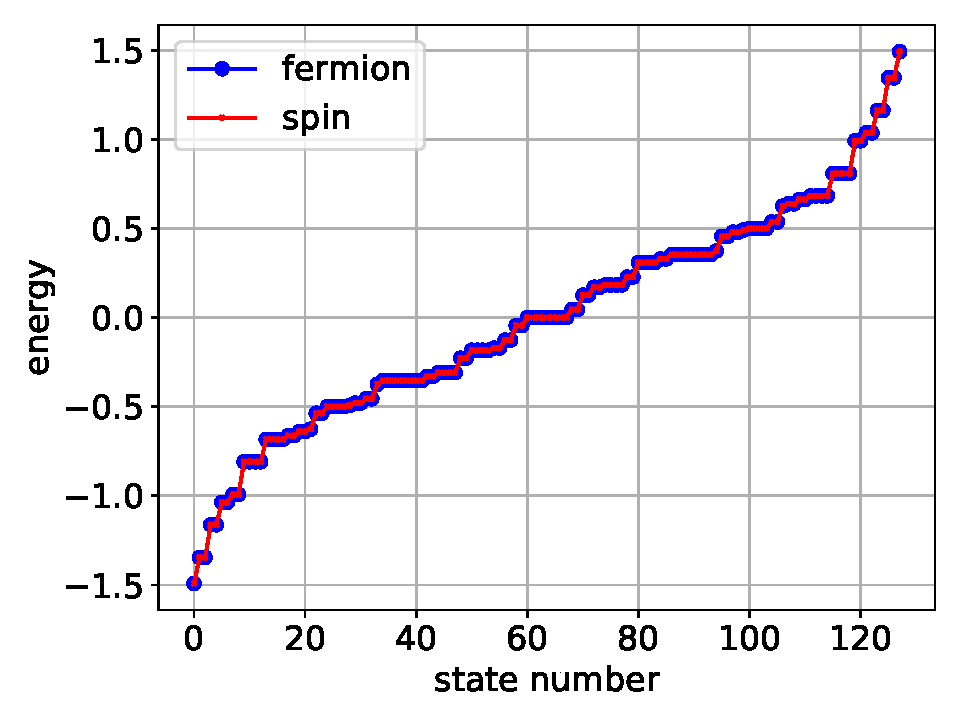
\includegraphics[width=\textwidth]{JW_PBC.pdf}
		\caption{negative spin inversion/PBC sector}
	\end{subfigure}
	\begin{subfigure}[b]{0.496\textwidth}
		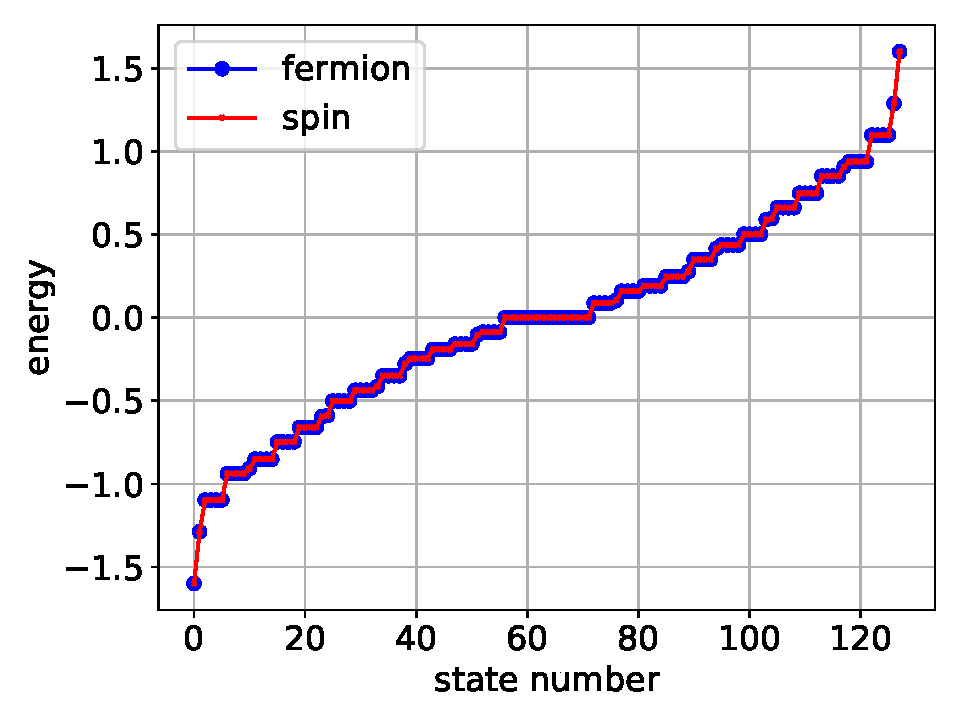
\includegraphics[width=\textwidth]{JW_APBC.pdf}
		\caption{positive spin inversion/APBC sector}
	\end{subfigure}
	\caption{\label{fig:JW} Comparison of the spectra of the spin and fermion representation of the transverse field Ising Hamiltonian in the spin~\eqref{eq:TFIM} and fermion~\eqref{eq:TFIM_fermion} representations. The degeneracy is the spectrum is due to the remaining parity and momentum conservations which are not taken into account (see text). The parameters are $J=1.0$, $h=\sqrt{2}$, and $L=8$.}  
\end{figure} 

\noindent\emph{Code Analysis---}We begin by loading the QuSpin operator and basis constructors, as well as some standard Python libraries. 
\lstinputlisting[firstline=1, lastline=4]{\JWcode}
First, we define the models parameters.
\lstinputlisting[firstline=5, lastline=8]{\JWcode}
We have to consider two cases when computing the spectrum, as discussed in the theory section above. In one case, the fermionic system has PBC, while the spins are constrained to the negative spin inversion symmetry sector, while in the second -- the fermion model has APBC and the spin model is considered in the positive spin inversion sector. To this end, we introduce the variables \texttt{zblock} $\in\{\pm 1\}$ and \texttt{PBC} $\in\{\pm 1\}$, where \texttt{PBC} $=-1$ denotes APBC. Note than the only meaningful combinations are $($\texttt{zblock}, \texttt{PBC}$)=(-1,1),(1,-1)$.
\lstinputlisting[firstline=9, lastline=10]{\JWcode}
Within this loop, the code is divided to two independent parts: first, we compute the spectrum of the TFI system, and then -- that of the equivalent fermionic model. Let us discuss the spins. 
\lstinputlisting[firstline=11, lastline=11]{\JWcode}
In QuSpin, operators are stored as sparse lists. These lists contain two parts: (i) the lattice sites on which the operator acts together with the coupling strength, which we call a \emph{site-coupling} list, and (ii) the types of the operators involved, i.e.~\emph{operator-string}. For example, the operator $\mathcal{O}=g\sum_{j=0}^{L-1}\sigma^\mu_j$ can be uniquely represented by the site-coupling list \texttt{[[g,0],[g,1],$\dots$,[g,L-1]]}, and the information that it is the Pauli matrix $\mu$. The components lists are nothing but the tuples of the field strength and the site index \texttt{[g,j]}. It is straightforward to generalise this to non-uniform fields \texttt{g$\to $g[j]}. Similarly, any two-body operator $\mathcal{O}=J_{zz}\sum_{j=0}^{L-1}\sigma^\mu_j\sigma^\nu_{j+1}$ can be fully represented by the two sites it acts on, and its coupling strength: \texttt{[J,j,j+1]}. We then stack up these elementary lists together into a the site-coupling list: \texttt{[[J,0,1],[J,1,2],$\dots$,[J,L-2,L-1],[J,L-1,0]]}. 
\lstinputlisting[firstline=12, lastline=14]{\JWcode}
Notice the way we defined the periodic boundary condition for the spin-spin interaction using the modulo operator \texttt{\%}, which effectively puts a coupling between sites $L-1$ and $0$. We mention in passing that the above procedure generalises so one can define any multi-body local and nonlocal operator using QuSpin. 

In order to specify the types of the on-site single-particle operators, we use operator strings. For instance, the transverse field operator $\mathcal{O}=g\sum_{j=0}^{L-1}\sigma^x_j$ becomes \texttt{['x',h\_field]}, while the two-body interaction is \texttt{['zz',J\_zz]}. It is important to notice that the order of the letters in the operator string corresponds to the order the operators are listed in the site-coupling lists. Putting everything into one final list yields:  
\lstinputlisting[firstline=15, lastline=16]{\JWcode}
In QuSpin, the user can define both static and dynamic operators. Since this example does not require any time evolution, we postpone the explanation of how to use dynamic lists to Sec.~\ref{subsec:GP_dynamics}, and use an empty list instead.
\lstinputlisting[firstline=17, lastline=17]{\JWcode}
The last step before we can construct the Hamiltonian is to build the basis for it. This is done using the basis constructors. For spin systems, we use \texttt{spin\_basis\_1d} which allows to use the operator strings \texttt{'z','+','-'}, and for spin-$1/2$ additionally \texttt{'x','y'}. The first and required argument is the number of sites $L$. Optional arguments are used to parse symmetry sectors. For instance, if we want to construct an operator in the spin-inversion block with quantum number $+1$, we can conveniently do this using the flag \texttt{zblock=1}.
\lstinputlisting[firstline=18, lastline=19]{\JWcode} 
Having specified the static and dynamic lists, as well as the basis, building up the Hamiltonian is a one-liner, using the \texttt{hamiltonian} constructor. The first and second compulsory arguments are the static and dynamic list, respectively. Optional arguments include the \texttt{basis}, and the precision or data type \texttt{dtype}. If no basis is passed, the constructor uses \texttt{spin\_basis\_1d} by default. The default data type is \texttt{np.complex128}.
\lstinputlisting[firstline=20, lastline=21]{\JWcode} 
The Hamiltonian is stored as a sparse matrix for efficiency. It can be cast to a full array for a more convenient inspection using the attribute \texttt{H.toarray()}. To calculate its spectrum, we use the attribute $H.eigenvalsh()$, which returns all eigenvalues. Other attributes for diagonalisation were discussed in Example 0 [PUT link to github], c.f.~Ref.~\cite{weinberg_17_quspin}.
\lstinputlisting[firstline=22, lastline=23]{\JWcode}

Let us now move to the second part of the loop which defines the fermionic $p$-wave superconductor. We start by defining the site-coupling list local potential
\lstinputlisting[firstline=24, lastline=26]{\JWcode}
Let us ficus on the case of periodic boundary conditions \texttt{PBC=1} first. 
\lstinputlisting[firstline=27, lastline=27]{\JWcode}
In the fermion model, we have two types of two-body terms: hopping terms $c^\dagger_{i}c_{i+1} - c_{i}c^\dagger_{i+1}$, and pairing terms $c^\dagger_{i}c^\dagger_{i+1} - c_{i}c_{i+1}$. While QuSpin allows any ordering of the operators, for te sake of completeness we set a convention: the site indices grows to the right. Do to the opposite signs in the terms resulting from the fermion statistics, we have to code the site-coupling lists for all four terms separately. This is analogous to the spin-spin interaction above:
\lstinputlisting[firstline=28, lastline=32]{\JWcode}
To construct a fermionic operator, we make use of the fermion basis constructor \texttt{fermion\_basis\_1d}. This Once again, we pass the number of sites \texttt{L}. As we explained in the analysis above, we need to consider all odd particle number sectors in the case of PBC. This is done by specifying the particle number sector \texttt{Nf}. 
\lstinputlisting[firstline=33, lastline=34]{\JWcode}

In the case of APBC, we first construct all two-body site-coupling lists as if the boundaries were open, and supplement the APBC links in the end:
\lstinputlisting[firstline=35, lastline=45]{\JWcode}
The definition of the basis is the same, except that this time, we need all even particle number sectors:
\lstinputlisting[firstline=46, lastline=47]{\JWcode}

As before, we need to specify the type of operators that go in the Hamiltonian using operator string lists. The \texttt{fermion\_basis\_1d} class accepts the following strings \texttt{'+','-','n'}, and additionally the particle-hole symmetrised density operator \texttt{'z'} $=n-1/2$. The static and dynamic lists read as
\lstinputlisting[firstline=48, lastline=50]{\JWcode}
Constructing and diagonalising the fermion Hamiltonian is the same as for the spin-$1/2$ system. Note that one can disable the automatic built-in checks for particle conservation \texttt{check\_pcon=False} and all other symmetries \texttt{check\_symm=False} if one wishes to suppress the checks. 
\lstinputlisting[firstline=51, lastline=55]{\JWcode}

The complete code including the lines that produce Fig.~\ref{fig:JW} is available in Example Code~\ref{code:ex4}.



\subsection{Free Particle Systems: the Fermionic SSH Chain}

\label{subsec:SSH_model}

This example shows how to
\begin{itemize}
	\item construct free-particle Hamiltonians in real space,
	\item implement translation invariance with a two-site unit cell and construct the single-particle Hamiltonian in momentum space in block-diagonal form,
	\item compute non-equal time correlation functions,
	\item ...
\end{itemize}

\noindent\emph{Physics Setup---}The Su-Schrieffer-Heeger (SSH) model of a free-particle on a dimerised chain is widely used to introduce the concept of edge states, topology, Berry phase, etc., in one spatial dimension. The Hamiltonian is given by
\begin{eqnarray}
H = \sum_{j=0}^{L-1} -(J+(-1)^j\delta J)\left(c_jc^\dagger_{j+1} - c^\dagger_{j}c_{j+1}\right) + \Delta(-1)^jn_j, 
\label{eq:SSH}
\end{eqnarray}
where $\{c_i,c^\dagger_j\}=\delta _{ij}$ obey fermionic commutation relations. The uniform part of the hopping matrix element is $J$, $\delta J$ defines the bond dimerisation, and $\Delta$ is the staggered potential. We assume periodic boundary conditions.

Below, we show how one can use QuSpin to study the physics of free fermions in the SSH chain. One way of doing this would be to work in the many-body (Fock space) basis, see Sec.~???. However, whenever the particles are non-interacting, the exponential scaling of the Hilbert space dimension with the number of lattice sites imposes an artificial limitation on the system sizes one can do. Luckily, with no interactions present, the many-body wave functions factorise in a product of single-particle states. Hence, it is possible to study the behaviour of many free bosons and fermions by simulating the physics of a single particle.

Making use of translation invariance, a straightforward Fourier transformation to momentum space, $a_k = \sqrt{2/L}\sum_{j\ \mathrm{even}}^{L-1} \mathrm e^{-i k j}c_{j}$ and $b_k = \sqrt{2/L}\sum_{j\ \mathrm{odd}}^{L-1}\mathrm e^{-i k j} c_{j}$, casts the SSH Hamiltonian in the following form
\begin{equation}
H \!=\! \sum_{k\in\mathrm{BZ'}} (a^\dagger_k,b^\dagger_k)^t
\left(\begin{array}{cc}
\Delta & -(J+\delta J)\mathrm e^{-i k} - (J-\delta J)\mathrm e^{+i k} \\
-(J+\delta J)\mathrm e^{+i k} - (J-\delta J)\mathrm e^{-i k} & -\Delta
\end{array}
\right)
\left(\! \begin{array}{c}
a_k\\
b_k
\end{array}
\!\right),
\end{equation}
where the reduced Brillouin zone is defined as $\mathrm{BZ'}=[-\pi/2,\pi/2)$. We thus see that the Hamiltonian reduces further to a set of independent $2\times 2$ matrices. The spectrum of the SSH model is gapped, see Fig.~???.

Since we are dealing with free fermions, the ground state is the Fermi sea, $|\mathrm{FS}\rangle$, defined by filling up the lowest band completely. We are interested in measuring the real-space non-equal time correlation function
\begin{equation}
C_{ij}(t) = \langle \mathrm{FS}|n_i(t)n_j(0)|\mathrm{FS}\rangle = \langle \mathrm{FS}(t)|n_i(0)\underbrace{U(t,0)n_j(0)|\mathrm{FS}\rangle}_{|\mathrm{nFS}(t)\rangle}.
\end{equation}
For simplicity, let us focus on a single unit cell. Figure~??? shows the time evolution of $C_{AA}(t)$ and $C_{AB}(t)$. 

\noindent\emph{Code Analysis---}...
\lstinputlisting[firstline=1, lastline=55]{\JWcode}

The complete code including the lines that produce Fig.~\ref{fig:example3} is available in Example Code~\ref{code:ex3}.







\subsection{Fermionic Many-body Localization}
\label{subsec:Fermion_MBL}

This example shows how to:
\begin{itemize}
	\item construct Hamiltonians for spinful fermions using the tensor\_basis class.
	\item how to use ops\_dict class to construct Hamiltonians with varying parameters.
	\item use new basis functionality to construct simple product states
	\item use obs\_vs\_time functionality to measure observables as a function of time
\end{itemize}

A class of exciting new problems in the field of non-equalibrium physics are that of the Many-body localzation (MBL) transition. The MBL transition is a dynamical phase transition in the eigenstates of a many-body Hamiltonian. Driven primarily by quenched disorder, the transition occurs is distinguished by ergodic eigenstates in the weak disorder limit and non-ergodic eigenstates in the strong disorder limit. The MBL phase is reminiscent of integrable systems as one can construct quasi-local integrals of motion in the MBL phase, but these integrals of motion are much more robust in the sense that they are not sensitive to small perturbations are is the case in many classes of integrable systems[CITE MBL misc].

Motivated by some recent experiments in cold atomic gasses [CITE Bloch MBL exp] we explore MBL in the context of fermions using QuSpin. The model we will consider is the Fermi-Hubbard model with quenched random disorder which has the following Hamiltonian:
\begin{equation}
	H = -J\sum_{\sigma,i=0}^{L-1} c^\dagger_{\sigma i}c_{\sigma i+1} - c_{\sigma i}c^\dagger_{\sigma i+1} +U\sum_{i=0}^L n_{\uparrow i}n_{\downarrow i} + \sum_{\sigma, i=0}^L V_i n_{\sigma i}\label{eq:FH_ham}
\end{equation}
where $c_{\sigma i}$ and $c^\dagger_{\sigma i}$ is a ferminoic creation and annihilation operators on site $i$ for spin $\sigma$ respectively. We will work in the sector of 1/4 filling for both up and down spins. Preparing an initial configuration of fermions of alternating spin on every other site, we will then measure the sublattice imbalance:
\begin{equation}
	I = (N_A-N_B)/N_\mathrm{tot}
\end{equation}
where $A$ and $B$ refer to the different sublattices of the chain and $N$ is the particle number operator. evolving with Hamiltonian~\eqref{eq:FH_ham} we will calculate its value which will tell us something about the ergodicity(or lack there of) of the Hamiltonian. If the Hamiltonian is ergodic then this quantity will decay to $0$ in the limit $t\rightarrow\infty$ as one would expect in equilibrium while if the Hamiltonian is MBL then some memory of its initial condition will be retained, and therefore this quantity will be non-zero even at infinite times.

Because the Hilbert space dimension grows so quickly for this Hamiltonian we will only consider the dynamics after a finite amount of time, and even with this it is a fairly long calculation to do $L>10$. 

\begin{figure}[t!]
	\centering
	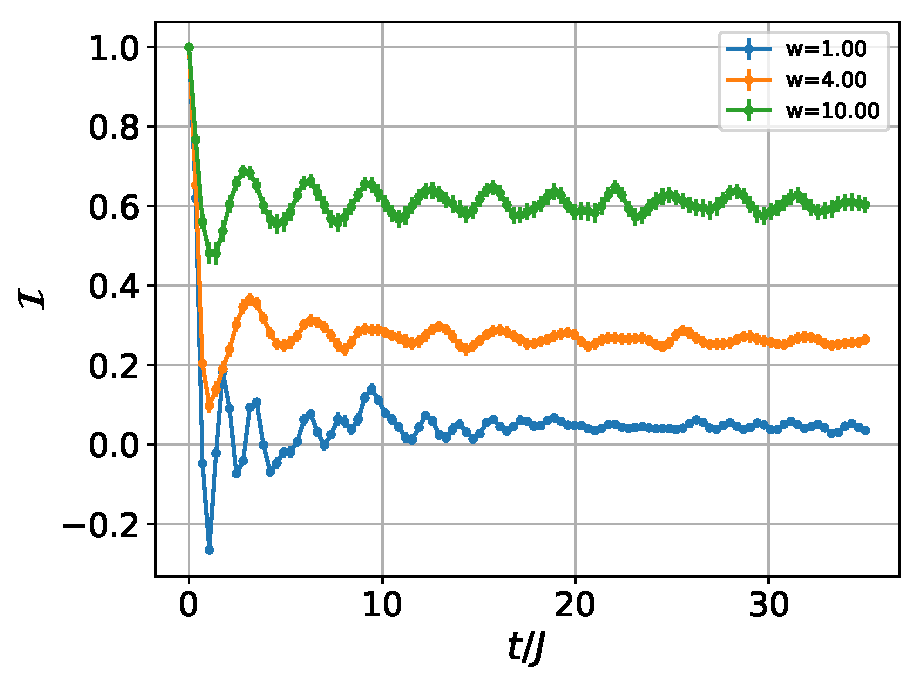
\includegraphics[width=0.5\textwidth]{fermion_MBL.pdf}
	\caption{Sublattice imbalance $I$ as a function of time averaged over 100 disorder realizations for different disorder strengths. This data was taken on a chain of length $L=8$.}
\end{figure}

\noindent\emph{Code Analysis---}...
\lstinputlisting[firstline=1, lastline=55]{\MBLcode}







\subsection{Bose-Hubbard Model on Translationally Invariant Ladder}
\label{subsec:Bose_Ladder}

This example shows how to:
\begin{itemize}
	\item construct Hamiltonians for bosonic systems.
	\item construct ladder Hamiltonians.
	\item using block\_ops class to evolve over several symmetry sectors at once.
	\item measure entanglement entropy of ladder.
\end{itemize}

\noindent{\emph{Physics Setup---}}In this example we will use QuSpin to solve the dynamics of the Bose-Hubbard model (BHM) on a ladder geometry. The BHM is a minimal model of interacting bosons which is experimentally realizable in cold atom experiments [CITE]. The Hamiltonian is given by:
\begin{equation}
	H_\mathrm{BHM} = -J\sum_{\langle ij\rangle} a_i^\dagger a_j + \mathrm{h.c.} + U\sum_{i}n_i(n_i-1)\label{eq:BHM_ham}
\end{equation} 
where $a_i$ and $a^\dagger_i$ are bosonic creation and annihilation operators on site $i$ respectively and the sum $\langle ij\rangle$ is a sum over nearest neighbors on Ladder. We will consider a half filled ladder of length $L$ with $N=2L$ sites. We will perform a quench where the system starts out in a random product state and let it evolve with Hamiltonian~\eqref{eq:BHM_ham}. We will restrict the local Hilbert space to allow at most 2-particles on a site which is valid in the large $U$ limit. This model is not integrable and so we expect that the system will eventually thermalize so that the occupation is roughly uniform over the entire system. On top of measuring the local density we will also measure the entanglement entropy between the legs of the ladder.

If we consider a translational invariant ladder that implies the Hamiltonian factorizes into different many-body momentum blocks similar to what was discussed in Sec.~\ref{subsec:SSH_model} but slightly different as we consider translations of the many-body fock states as opposed to the single particle states[CITE Anders review]. In this section instead of projecting the operators to momentum space as was done in Sec.~\ref{subsec:SSH_model}, we will project the wavefunction to the different symmetry sectors and evolve each of the projections separately under the Hamiltonian for that symmetry sector. Then each of the Block wavefunctions are projected back to the local Fock space basis and summed to recover the evolve state which one can then look at local quantities like the density and entanglement.
\begin{figure}[t!]
	\centering
	\begin{subfigure}[a]{0.496\textwidth}
		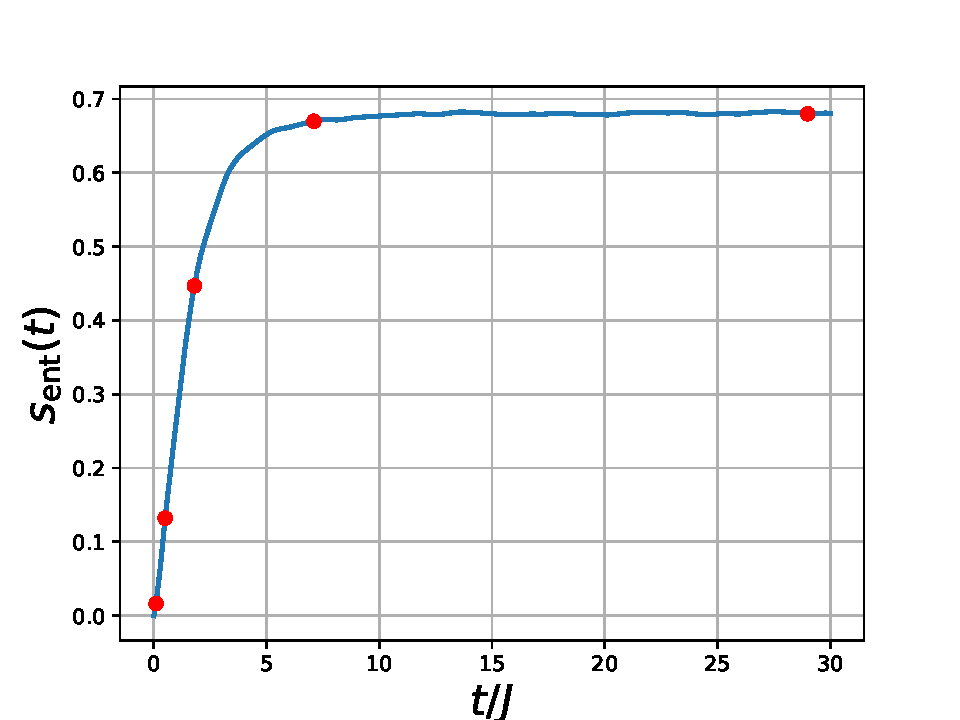
\includegraphics[width=0.9\textwidth]{boson_entropy.pdf}
		\caption{Entanglement entropy density between the two legs of the ladder as a function of time.}
	\end{subfigure}
	\begin{subfigure}[b]{0.496\textwidth}
		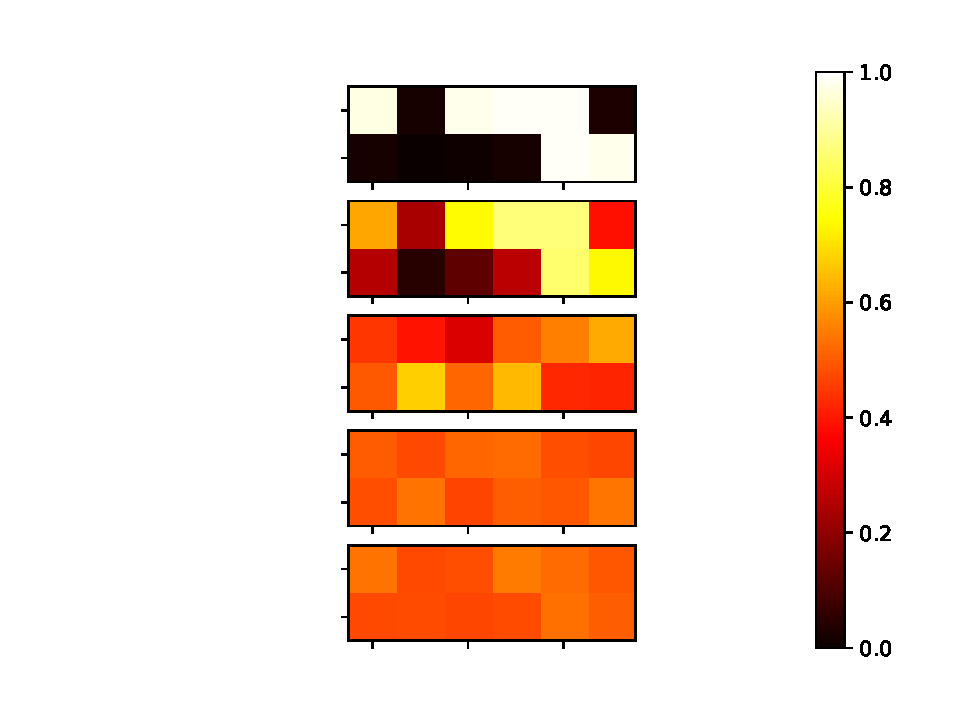
\includegraphics[width=0.9\textwidth]{boson_density.pdf}
		\caption{local density of bosons as a function of time. Later times appearing farther down the page.}
	\end{subfigure}
	\caption{Showing results from the quench in the BHM. plot (a) shows the half-ladder entanglement entropy density and plot (b) shows the local density on each site as a function of time. The red dots on the entanglement plot shows the time points where the density plots are taken. For this data was taken with $J=1$ and $U=10$.}
\end{figure}

\noindent\emph{Code Analysis---} Just as in the previous examples we start out our python script by loading some essential modules needed for the calculation
\lstinputlisting[firstline=3, lastline=6]{\BHLcode}
Next we set up the model parameters defining the length of the ladder \texttt{L} chain number of sites \texttt{N=2*L} as well as filling factor for the bosons \texttt{nb}, and the maximum number of states per site \texttt{sps}. The hopping matrix elements $J_\perp$, $J_{\parallel,1}$, and $J_{\parallel,2}$ (see Fig.~\ref{fig:BHL_geometry}\cyan{create figure showing ladder and couplings etc...}), correspond to the python script are variables \texttt{J\_perp}, \texttt{J\_par\_1}, and \texttt{J\_par\_2} respectively.
\lstinputlisting[firstline=44, lastline=52]{\BHLcode} Next we set up the times at which we would like to solve the Schrödinger equation. Due to the same restrictions on the exponential solver discussed Sec .~\ref{subsec:Fermion_MBL} we will only consider time points which are linearly spaced defined by the variables \texttt{start},\texttt{stop}, and \texttt{num}
\lstinputlisting[firstline=53, lastline=55]{\BHLcode}
For bosonic systems we have \texttt{'+'},\texttt{'-'}, and \texttt{'n'} as possible operators to use. In order to set up the Hubbard local interaction we must define two coupling lists for the $U\sum_{i} n_i^2$ and the $-U\sum_{i} n_i$:
\lstinputlisting[firstline=56, lastline=58]{\BHLcode}
We also define the hopping lists
\lstinputlisting[firstline=59, lastline=63]{\BHLcode}
where we use the \texttt{[...].extend([...])} method to concatenate two lists together\footnote{Note that the \texttt{extend} function is done inplace so if you try to do \texttt{new\_list=list.extend(other\_list)}, \texttt{new\_list} will be \texttt{None} and \texttt{list} will have all of the elements of \texttt{other\_list} appended to it.}. The way the ladder is defined, the even sites correspond to the bottom side while the odds sites are the top part of the ladder, therefore the hopping on the bottom/top runge is defined by \texttt{[J\_par\_...,i,(i+2)\%N]}, while hopping from top to bottom is defined by \texttt{[J\_perp,i,(i+1)\%N]}. Finally we can define the static and dynamic lists
\lstinputlisting[firstline=64, lastline=71]{\BHLcode}
which we will not use to construct a \texttt{hamiltonian} object but instead we will use the \texttt{block\_ops} class. The purpose of \texttt{block\_ops} is to provide a simple interface for solving the Schrödinger equation when an initial state may not obey the symmetries of the Hamiltonian which is generating the dynamics. We have seen an example of this in Sec.~\ref{subsec:SSH_model} when trying to measure non-equal time correlation functions of local operators, while in this section we explicitly start out with a state which does not obey translational invariance. Before we construct the \texttt{block\_ops} let us first define a few things which will be used to construct the \texttt{block\_ops} object
\lstinputlisting[firstline=72, lastline=82]{\BHLcode}
Firstly, \texttt{blocks} is a list of dictionaries which define the different symmetry sectors to evolve the initial state over\footnote{\texttt{block\_ops} will not evolve a particular symmetry sector if the projection is 0.}.


\subsection{The Gross-Pitaevskii Equation and Nonlinear Time Evolution}
\label{subsec:GP_dynamics}

This example shows how to
\begin{itemize}
	\item simulate time-dependent nonlinear equations of motion
	\item use imaginary time dynamics to find a lowest energy configuration
	\item ...
\end{itemize}

\noindent\emph{Physics Setup---}The Gross-Pitaevskii wave equation (GPE) has been shown to govern the physics of weakly-interacting bosonic systems. It constitutes the starting point for studying Bose-Einstein condensates, but can also appear in non-linear optics, and represents the natural description of Hamiltonian mechanics in the wave picture. One of its characteristic features is that it exhibits chaotic classical dynamics, a physical manifestation of the presence of a cubic non-linear term.

Here, we study the time-dependent GPE on a one-dimensional lattice:
\begin{eqnarray}
i\partial_t\psi_j(t) &=& -J\left( \psi_{j-1}(t) + \psi_{j+1}(t)\right) + \frac{1}{2}\omega_\mathrm{trap}(t)(j-j_0)^2\psi_j(t) + U|\psi_j(t)|^2\psi_j(t), \nonumber \\
\omega_\mathrm{trap}(t)&=&(\omega_f-\omega_i)t/t_\mathrm{ramp}+ \omega_i
\label{eq:GPE}
\end{eqnarray}
where $J$ is the hopping matrix element, $\omega_\mathrm{trap}(t)$ -- the slowly-varying time-dependent harmonic trap `frequency' over a time scale $t_\mathrm{ramp}$, and $U$ -- the interaction strength. The lattice sites are labelled by $j=0,\dots,L-1$, and $j_0$ is the centre of the 1d chain. We set the lattice constant to unity, and use open boundary conditions.

Whenever $U=0$, the system is non-interacting and the GPE reduces to the Heisenberg EOM for the bosonic field operator $\hat\psi_j(t)$. Thus, for the purposes of using QuSpin to simulate the GPE, it is instructive to cast Eq.~\eqref{eq:GPE} in the following generic form
\begin{equation}
i\partial_t\vec{\psi}(t) = H_\mathrm{sp}(t)\vec{\psi}(t) + U \vec{\psi}^*(t)\circ \vec{\psi}(t)\circ \vec{\psi}(t), 
\end{equation}  
where $[\vec{\psi}(t)]_j = \psi_j(t)$, and $\circ$ represents the element-wise multiplication 
\begin{equation*}
\vec{\psi}(t)\circ \vec{\phi}(t) = \bigg(\psi_0(t)\phi_0(t), \psi_1(t)\phi_1(t),\dots, \psi_{L-1}(t)\phi_{L-1}(t) \bigg)^t.
\end{equation*}
The time-dependent single-particle Hamiltonian in real space is represented as an $L\times L$ matrix, $H_\mathrm{sp}(t)$, which comprises the hopping term, and the harmonic trap.

We want to initiate the time-evolution of the system at $t=0$ in its lowest energy state. To this end, we can define a `ground state' for the GPE equation, in terms of the configuration which minimises the energy of the system:
\begin{eqnarray}
\vec\psi_\mathrm{GS} &=& \inf_{\vec{\psi}} \bigg( \vec{\psi}^t H_\mathrm{sp}(0)\vec{\psi} + \frac{U}{2}\sum_{j=0}^{L-1}|\psi_j|^4\bigg),\nonumber\\
&=&\inf_{\psi_j} \bigg(\sum_{j=0}^{L-1} -J(\psi_{j+1}^*\psi_j + \mathrm{c.c.}) + \frac{1}{2}\omega_\mathrm{trap}(0)|\psi_j|^2 + \frac{U}{2}|\psi_j|^4\bigg).
\end{eqnarray} 
One way to find the configuration $\vec\psi_\mathrm{GS}$, is to solve the GPE in imaginary time ($it\to \tau$), which induces exponential decay in all modes of the system, except for the lowest-energy state. In doing so, we keep the norm of the solution fixed:
\begin{eqnarray}
\label{eq:GPE_imag}
\partial_{\tau}\vec\varphi(\tau) &=& -\bigg[H_\mathrm{sp}(0)\vec\varphi(\tau) + U \vec\varphi^*(\tau)\circ \vec\varphi(\tau)\circ \vec\varphi(\tau)\bigg],\qquad ||\vec\varphi(\tau)||=\mathrm{const.},\nonumber\\
\vec{\psi}_\mathrm{GS} &=& \lim_{\tau\to\infty}\vec\varphi(\tau)
\end{eqnarray}
Once we have the initial state $\vec\psi_\mathrm{GS}$, we evolve it according to the time-dependent GPE, Eq.~\eqref{eq:GPE}, and track down the time evolution of the condensate density $\rho_j(t)=|\psi_j(t)|^2$. Fig.~??? shows the result.

\noindent\emph{Code Analysis---}In the following, we demonstrate how one can code the above physics using QuSpin. As usual, we begin by loading the necessary packages
\lstinputlisting[firstline=1, lastline=6]{\GPcode}
Next, we define the model parameters. We distinguish between static parameters and dynamic parameters -- those involved in the trap widening.
\lstinputlisting[firstline=7, lastline=21]{\GPcode}
In order to do time evolution, we define the trap widening protocol from Eq.~\eqref{eq:GPE}. Since we want to make use of QuSpin's time-dependent operator features, the first argument must be the time vector, followed by all protocol parameters. These same parameters are then listed in the variable \texttt{ramp\_args}.
\lstinputlisting[firstline=22, lastline=26]{\GPcode}
With this, we are ready to construct the single-particle Hamiltonian. The first step is to define the site-coupling lists, and the static and dynamic lists. Note that the dynamic list, which defines the harmonic potential in the single-particle Hamiltonian, contains four elements: apart from the operator string and the corresponding site-coupling list, the third and fourth elements are the time-dependent function \texttt{ramp} and its arguments \texttt{ramp\_args} in this order.
\lstinputlisting[firstline=27, lastline=33]{\GPcode}
To create a single-particle Hamiltonian, we choose to use the bosonic basis constructor \texttt{boson\_basis\_1d} specifying the number sector to \texttt{Nb=1} boson for the entire lattice, and a local Hilbert space of \texttt{sps=2} states per site (empty and filled). 
\lstinputlisting[firstline=34, lastline=35]{\GPcode}
Then we call the \texttt{hamiltonian} constructor to build the single-particle matrix. We can obtain the single-particle ground state without fully diagonalising the matrix by using the sparse diagonalisation attribute \texttt{Hsp.eigsh()}, with the options \texttt{k=1} and \texttt{'which'='SA'} which specify taking only one state starting from the bottom of the spectrum, i.e.~the ground state.	
\lstinputlisting[firstline=36, lastline=38]{\GPcode}
The next step in the program is to compute the ground state of the GPE using imaginary time evolution from Eq.~\eqref{eq:GPE_imag}. To this end, we first define the function \texttt{GPE\_imag\_time} which evaluate the RHS. It is required that the first argument for this function is (imaginary) time \texttt{tau}, followed by the state \texttt{phi}. All other arguments, such as the single-particle Hamiltonian and the interaction strength are listed last. Similar to before, we store these optional arguments in a list which we call \texttt{GPE\_params}. 
\lstinputlisting[firstline=39, lastline=47]{\GPcode}
Any initial value problem requires us to pick an initial state. In the case of imaginary evolution, this state can often be arbitrary, but needs to possess the same symmetries as the true GPE ground state. Here, we choose the ground state of the single-particle Hamiltonian for an initial state, and normalise it to one particle per site. We also define the imaginary time vector \texttt{tau}. This array has to contain sufficiently long times so that we make sure we obtain the long imaginary time limit $\tau\to\infty$, as required by Eq.~\eqref{eq:GPE_imag}. SInce imaginary time evolution is not unitary, QuSpin will be normalising the vector every $\tau$-step. Thus, one also needs to make sure these steps are small enough to avoid convergence problems of the ODE solver.
\lstinputlisting[firstline=48, lastline=51]{\GPcode}
Performing Imaginary time evolution is done using the \texttt{evolve()} method of the \texttt{measurements} tool. This function accepts an initial state \texttt{phi0}, initial time \texttt{tau[0]}, and a time vector \texttt{tau} and solves the user-defined ODE \texttt{GPE\_imag\_time}. The parameters of the ODE are passed using the keyword argument \texttt{f\_params=GPE\_params}. To ensure the normalisation of the state at each $\tau$-step we use the flag \texttt{imag\_time=True}. Real-valued output can be specified by \texttt{real=True}. Last, we request \texttt{evolve()} to create a generator object using the keyword argument \texttt{iterate=True}. Many of the keyword arguments of \texttt{evolve()} are the same as in the \texttt{H.evolve()} method of the \texttt{hamiltonian class}: for instance, one can choose a specific SciPy solver and its arguments, or the solver's absolute and relative tolerance. We refer the interested reader to the documentation, cf.~Sec.~\ref{app:doc}.
\lstinputlisting[firstline=52, lastline=54]{\GPcode}
Looping over the generator \texttt{phi\_tau} we have access to the solution, which we display in a form of a movie:
\lstinputlisting[firstline=55, lastline=72]{\GPcode}
Last, we use our GPE ground state, to time-evolve it in real time according to the trap widening protocol hard-coded into the single-particle Hamiltonian. We proceed analogously -- first we define the real-time GPE and the time vector. In defining the GPE function, we split the ODE into a time-independent static part and a time-dependent dynamic part. The single-particle Hamiltonian for the former is accessed using the \texttt{hamiltonian} attribute \texttt{Hsp.static} which returns a sparse matrix. We can then manually add the non-linear cubic mean-field interaction term. In order to access the time-dependent part of the Hamiltonian, and evaluate it, we loop over the dynamic list \texttt{Hsp.dynamic}, reading off the orresponding operator \texttt{Hd} together with the time-dependent function \texttt{f} which multiplies it, and its arguments \texttt{f\_args}. Last, we multiply the final ouput vector by the Schr\"odinger $-i$, which ensures the unitarity of for real-time evolution.
\lstinputlisting[firstline=73, lastline=86]{\GPcode}
To perform real-time evolution we once again use the \texttt{evolve()} function. This time, however, since the solution of the GPE is anticipated to be complex-valued, and because we do not do imaginary time, we do not need to pass the flags \texttt{real} and \texttt{imag\_time}. Instead, we decided to show the flags for the relative and absolute tolerance of the solver. 
\lstinputlisting[firstline=87, lastline=88]{\GPcode}
Finally, we can enjoy the movie displaying real-time evolution
\lstinputlisting[firstline=89, lastline=107]{\GPcode}

The complete code including the lines that produce Fig.~\ref{fig:example8} is available in Example Code~\ref{code:ex8}.



\subsection{Integrability Breaking in Higher spin TFI model}

This example shows how to:
\begin{itemize}
	\item construct Hamiltonians for Higher spin operators.
	\item find ground state of a Hamiltonian
	\item use obs\_vs\_time function with costume user defined generator to calculate the expectation value of operators as a function of time.
	\item use the new functionality of the basis class to calculate the entanglement entropy for higher spin.
\end{itemize}

\noindent{\emph{Physics Setup---}} In the previous section we introduced the TFI model and showed how one can solve the problem using the Jordan-Wigner transformation. This transformation allows one to get an exact analytic solution to the Hamiltonian (when the system obeys translational invariance). The fact that this solution exists in deeply connected to the notion of Integrability which has implications of how the system responds to a periodic modulation [CITE]. For non-integrable system when periodic driving, energy is no longer conserved and so generically one would expect that the system will heat up to infinite temperature, while in an integrable system, even though energy is not conserved, there are an extensive number of other static conserved quantities which may be conserved under the drive. If this is the case, then the system will not heat up at long times, but instead reach some steady state. By simply taking the transverse field ising model and promoting the spin-1/2 operators to spin-1, there is no longer a simple mapping to a quadratic Hamiltonian and therefore the model is no longer integrable. Here we will show this explicitly by driving the two different systems and checking it they heat or not. To do this we will define two Hamiltonians
\begin{equation}
H_{zz} = -\sum_{i=0}^{L-1} S^z_iS^z_{i+1}, \qquad H_{x} = -\sum_{i=0}^{L-1}S^x_i
\end{equation}
and evolve the ferromagnetic ground state of $H_{zz}$ with the following piecewise periodic Hamiltonian:
\begin{equation}
H(t)=H_{zz} -\Omega\,\mathrm{sgn}\left(\cos(\Omega t)\right)H_x
\end{equation}
where $\Omega$ is the driving frequency and $T$ is the period. As the Hamiltonian obeys translation,parity and spin-inversion symmetries we will use this to speed up the evolution by working in the symmetry sector which contains the ground state. 

In order to measure the difference in heating between spin-1 and spin-1/2 we measure the expectation value of $H_{zz}$ as a function of time. This operator has a symmetric spectrum and so following ref.[CITE heading papers] we define $Q$:
\begin{equation}
Q(t) =\left\langle\psi(t)\left\vert\frac{ 2\left(H_{zz}-E_\mathrm{min}\right)}{E_\mathrm{max}-E_\mathrm{min}}\right\vert\psi(t)\right\rangle=\left\langle\psi(t)\left\vert\frac{ H_{zz}-E_\mathrm{min}}{-E_\mathrm{min}}\right\vert\psi(t)\right\rangle
\end{equation}
where the last equality comes from the symmetry of the spectrum: $E_\mathrm{max}=-E_\mathrm{min}$. This quantity is defined such that an infinite temperature state has $Q=1$. Another measure of heating we will use is the entanglement entropy density
\begin{equation}
s_\mathrm{ent}(t) = -\frac{1}{|\mathrm{A}|}\mathrm{tr}_{\mathrm{A}}\left[\rho_\mathrm{A}(t)\log\rho_\mathrm{A}(t)\right], \qquad \rho_\mathrm{A}(t) = \mathrm{tr}_{\mathrm{A^c}} |\psi(t)\rangle\langle\psi(t)|
\end{equation}
of subsystem A, defined to contain the left half of the chain and $|\mathrm{A}|=L/2$. We denoted the reduced density matrix of subsystem A by $\rho_\mathrm{A}$, and $\mathrm{A^c}$ is the complement of A. 
\begin{figure}
	\begin{subfigure}[a]{0.496\textwidth}
		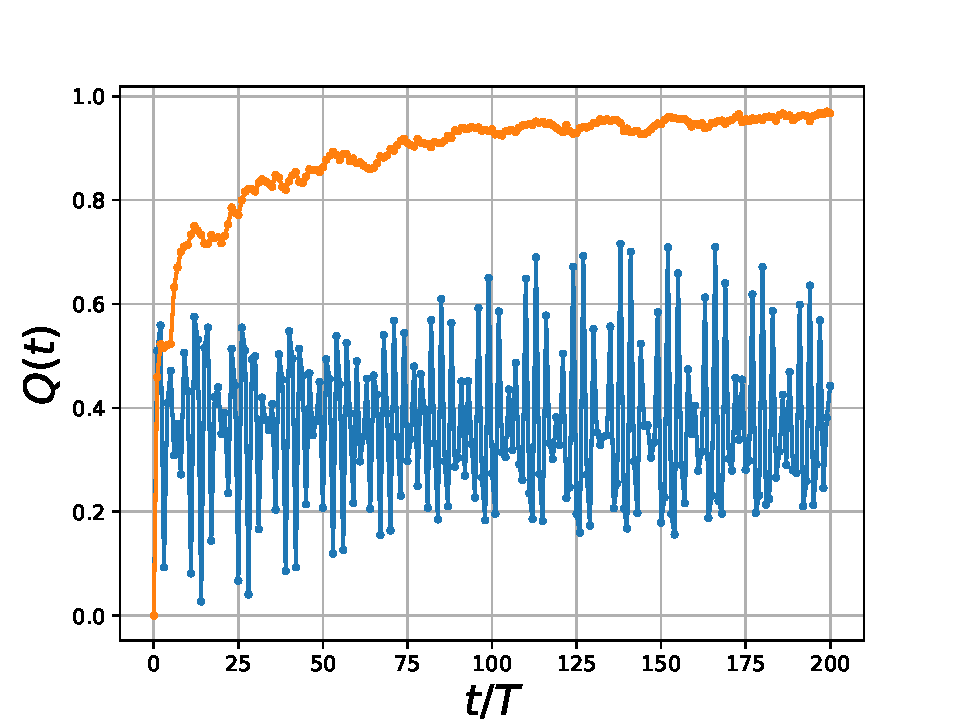
\includegraphics[width=0.9\textwidth]{TFIM_Q.pdf}
		\caption{$Q(t)$ for $t=nT$}
	\end{subfigure}
	\begin{subfigure}[b]{0.496\textwidth}
		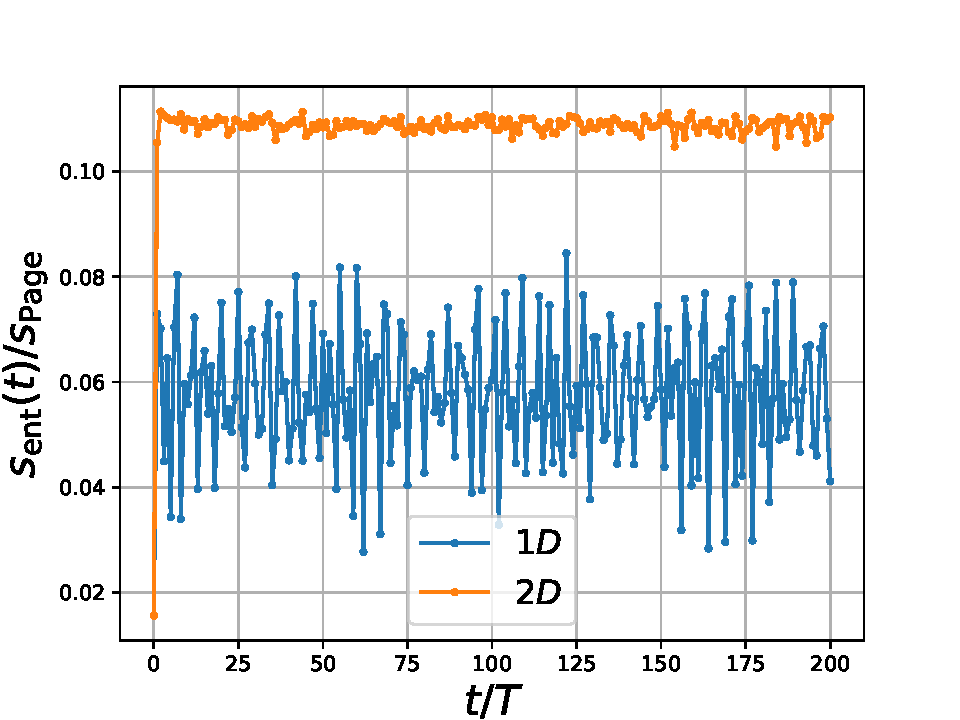
\includegraphics[width=0.9\textwidth]{TFIM_S.pdf}
		\caption{$s_\mathrm{ent}(t)/s_\mathrm{Page}$ for $t=nT$}
	\end{subfigure}
	\caption{Comparing the dynamics of $Q(t)$ (a) and $s_\mathrm{ent}(t)$ (b) for $S=1$ (orange) and $S=1/2$ (blue) at stroboscopic times ($t=nT$). For $S=1$ and $S=1/2$ we take $L=11$ and $18$ respectively as to make sure the many-body Hilbert spaces have roughly the same number of state. $s_\mathrm{ent}$ is normalized by the Page entropy per site[CITE Page]. Note that for both systems $\Omega=4$.}
\end{figure}

\noindent\emph{Code Analysis---}...
\lstinputlisting[firstline=1, lastline=55]{\Spincode}

The complete code including the lines that produce Fig.~\ref{fig:example3} is available in Example Code~\ref{code:ex3}.



\section{New Horizons for QuSpin}
\label{sec:outro}

\begin{itemize}
	\item 2D lattices
	\item single-particle Hamiltonian class
	\item Liouville dynamics
\end{itemize}
 

We would much appreciate it if the users could report bugs using the \href{https://github.com/weinbe58/qspin/issues}{issues} forum in the QuSpin online repository.


\section*{Acknowledgements}
We would like to thank L.~Pollet, M.~Kolodrubetz, S.~Capponi ... for various stimulating discussions and for providing comments on the draft. The authors are pleased to acknowledge that the computational work reported on in this paper was performed on the Shared Computing Cluster which is administered by \href{http://www.bu.edu/tech/support/research/}{Boston University's Research Computing Services}. The authors also acknowledge the Research Computing Services group for providing consulting support which has contributed to the results reported within this paper. We would also like to thank \href{https://github.com/}{Github} for providing the online resources to help develop and maintain this project. 

% TODO: include funding information
\paragraph{Funding information}
This work was supported by ???
\begin{appendix}
	
\section{Installation Guide in a Few Steps}
	\label{app:install}
	
	QuSpin is currently only being supported for Python 2.7 and Python 3.5 and so one must make sure to install this version of Python. We recommend the use of the free package manager \href{https://www.continuum.io/downloads}{Anaconda} which installs Python and manages its packages. For a lighter installation, one can use \href{http://conda.pydata.org/miniconda.html}{miniconda}.
	
	\subsection{Mac OS X/Linux}
	To install Anaconda/miniconda all one has to do is execute the installation script with administrative privilege. To do this, open up the terminal and go to the folder containing the downloaded installation file and execute the following command: 
	\begin{lstlisting}[numbers=none,keywordstyle=\ttfamily]
	$ sudo bash <installation_file>
	\end{lstlisting}
	You will be prompted to enter your password. Follow the prompts of the installation. We recommend that you allow the installer to prepend the installation directory to your PATH variable which will make sure this installation of Python will be called when executing a Python script in the terminal. If this is not done then you will have to do this manually in your bash profile file:
	\begin{lstlisting}[numbers=none,keywordstyle=\ttfamily]
	$ export PATH="path_to/anaconda/bin:$PATH"
	\end{lstlisting}
	
	\underline{\bf Installing via Anaconda.}---Once you have Anaconda/miniconda installed, all you have to do to install QuSpin is to execute the following command into the terminal: 
	\begin{lstlisting}[numbers=none,keywordstyle=\ttfamily]
	$ conda install -c weinbe58 quspin
	\end{lstlisting}
	If asked to install new packages just say `yes'. To keep the code up-to-date, just run this command regularly. 
	
	\underline{\bf Installing Manually.}---Installing the package manually is not recommended unless the above method failed. Note that you must have the Python packages NumPy, SciPy, and Joblib installed before installing QuSpin. Once all the prerequisite packages are installed, one can download the source code from \href{https://github.com/weinbe58/qspin/tree/master}{github} and then extract the code to whichever directory one desires. Open the terminal and go to the top level directory of the source code and execute:
	\begin{lstlisting}[numbers=none,keywordstyle=\ttfamily]  
	$ python setup.py install --record install_file.txt
	\end{lstlisting}
	This will compile the source code and copy it to the installation directory of Python recording the installation location to \texttt{install\_file.txt}. To update the code, you must first completely remove the current version installed and then install the new code. The \texttt{install\_file.txt} can be used to remove the package by running:  
	\begin{lstlisting}[numbers=none,keywordstyle=\ttfamily]  
	$ cat install_file.txt | xargs rm -rf. 
	\end{lstlisting}
	
	\subsection{Windows}
	To install Anaconda/miniconda on Windows, download the installer and execute it to install the program. Once Anaconda/miniconda is installed open the conda terminal and do one of the following to install the package:
	
	\underline{\bf Installing via Anaconda.}---Once you have Anaconda/miniconda installed all you have to do to install QuSpin is to execute the following command into the terminal: 
	\begin{lstlisting}[numbers=none,keywordstyle=\ttfamily]
	> conda install -c weinbe58 quspin
	\end{lstlisting}
	If asked to install new packages just say `yes'. To update the code just run this command regularly. 
	
	\underline{\bf Installing Manually.}---Installing the package manually is not recommended unless the above method failed. Note that you must have NumPy, SciPy, and Joblib installed before installing QuSpin. Once all the prerequisite packages are installed, one can download the source code from \href{https://github.com/weinbe58/qspin/tree/master}{github} and then extract the code to whichever directory one desires. Open the terminal and go to the top level directory of the source code and then execute:  
	\begin{lstlisting}[numbers=none,keywordstyle=\ttfamily]
	> python setup.py install --record install_file.txt
	\end{lstlisting}
	This will compile the source code and copy it to the installation directory of Python and record the installation location to \texttt{install\_file.txt}. To update the code you must first completely remove the current version installed and then install the new code. 
	
	
	\section{Basic Use of Command Line to Run Python}
	\label{app:cmd_line}
	
	In this appendix we will review how to use the command line for Windows and OS X/Linux to navigate your computer's folders/directories and run the Python scripts.
	
	\subsection{Mac OS X/Linux}
	Some basic commands:
	
	\begin{itemize}
		\item change directory:
		\begin{lstlisting}[numbers=none,keywordstyle=\ttfamily]
		$ cd < path_to_directory >
		\end{lstlisting}
		\item list files in current directory:
		\begin{lstlisting}[numbers=none,keywordstyle=\ttfamily]
		$ ls 
		\end{lstlisting}
		list files in another directory:
		\begin{lstlisting}[numbers=none,keywordstyle=\ttfamily]
		$ ls < path_to_directory >
		\end{lstlisting}
		\item make new directory:
		\begin{lstlisting}[numbers=none,keywordstyle=\ttfamily]
		$ mkdir <path>/< directory_name >
		\end{lstlisting}
		\item copy file:
		\begin{lstlisting}[numbers=none,keywordstyle=\ttfamily]
		$ cp < path >/< file_name > < new_path >/< new_file_name >
		\end{lstlisting}
		\item move file or change file name:
		\begin{lstlisting}[numbers=none]
		$ mv < path >/< file_name > < new_path >/< new_file_name >
		\end{lstlisting}
		\item remove file:
		\begin{lstlisting}[numbers=none,keywordstyle=\ttfamily]
		$ rm < path_to_file >/< file_name >
		\end{lstlisting}
		
	\end{itemize}
	Unix also has an auto complete feature if one hits the TAB key. It will complete a word or stop when it matches more than one file/folder name. The current directory is denoted by "." and the directory above is "..".
	%
	Now, to execute a Python script all one has to do is open your terminal and navigate to the directory which contains the python script. To execute the script just use the following command:
	\begin{lstlisting}[numbers=none,keywordstyle=\ttfamily]
	$ python script.py
	\end{lstlisting}
	It's that simple!
	
	\subsection{Windows}
	Some basic commands:
	
	\begin{itemize}
		\item change directory:
		\begin{lstlisting}[numbers=none,keywordstyle=\ttfamily]
		> cd < path_to_directory >
		\end{lstlisting}
		\item list files in current directory:
		\begin{lstlisting}[numbers=none,keywordstyle=\ttfamily]
		> dir
		\end{lstlisting}
		list files in another directory:
		\begin{lstlisting}[numbers=none,keywordstyle=\ttfamily]
		> dir < path_to_directory >
		\end{lstlisting}
		\item make new directory:
		\begin{lstlisting}[numbers=none,keywordstyle=\ttfamily]
		> mkdir <path>\< directory_name >
		\end{lstlisting}
		\item copy file:
		\begin{lstlisting}[numbers=none,keywordstyle=\ttfamily]
		> copy < path >\< file_name > < new_path >\< new_file_name >
		\end{lstlisting}
		\item move file or change file name:
		\begin{lstlisting}[numbers=none,keywordstyle=\ttfamily]
		> move < path >\< file_name > < new_path >\< new_file_name >
		\end{lstlisting}
		\item remove file:
		\begin{lstlisting}[numbers=none,keywordstyle=\ttfamily]
		> erase < path >\< file_name >
		\end{lstlisting}
		
	\end{itemize}
	Windows also has a auto complete feature using the TAB key but instead of stopping when there multiple files/folders with the same name, it will complete it with the first file alphabetically. The current directory is denoted by "." and the directory above is "..".
	
	\subsection{Execute Python Script (any operating system)}
	%
	To execute a Python script all one has to do is open up a terminal and navigate to the directory which contains the Python script. Python can be recognised by the extension \texttt{.py}. To execute the script just use the following command:
	\begin{lstlisting}[numbers=none,keywordstyle=\ttfamily]
	python script.py
	\end{lstlisting}
	It's that simple!
	
	\newpage
	
	\section{Package Documentation}
	\label{app:doc}
	In QuSpin quantum many-body operators are represented as matrices. The computation of these matrices are done through custom code written in Cython. Cython is an optimizing static compiler which takes code written in a syntax similar to Python, and compiles it into a highly efficient C/C\texttt{++} shared library. These libraries are then easily interfaced with Python, but can run orders of magnitude faster than pure Python code~\cite{Cython}. The matrices are stored in a sparse matrix format using the sparse matrix library of SciPy~\cite{SciPy_package}. This allows QuSpin to easily interface with mature Python packages, such as NumPy, SciPy, any many others. These packages provide reliable state-of-the-art tools for scientific computation as well as support from the Python community to regularly improve and update them~\cite{NumPy,Python_computing_1,Python_computing_2,SciPy_package}. Moreover, we have included specific functionality in QuSpin which uses NumPy and SciPy to do many desired calculations common to ED studies, while making sure the user only has to call a few NumPy or SciPy functions directly. The complete up-to-date documentation for the package is available online under:\\
	
	\href{https://github.com/weinbe58/QuSpin/#quspin}{https://github.com/weinbe58/QuSpin/\#quspin}\\
	
	\newpage
	\section{Complete Example Codes}
	\label{app:scripts}
	
	In this appendix, we give the complete python scripts for the dix examples discussed in Sec.~\ref{sec:examples}. In case the reader has trouble with the TAB spaces when copying from the code environments below, the scripts can be downloaded from github at: \center{ \href{https://github.com/weinbe58/QuSpin/tree/master/examples}{https://github.com/weinbe58/QuSpin/tree/master/examples}}
	
	
	\lstinputlisting[label=code:ex4,caption=The Spectrum of the Transverse Field Ising Model and the Jordan-Wigner Transformation]{\JWcode}
	\newpage
	%\lstinputlisting[label=code:ex1,caption=Adiabatic Control of Parameters in MBL Phases]{example1.py}
	%\newpage
	%\lstinputlisting[label=code:ex2,caption=Heating in Periodically Driven Spin Chains]{example2.py}
	%\newpage
	\lstinputlisting[label=code:ex8,caption=The Gross-Pitaevskii Equation and Nonlinear Time Evolution]{\GPcode}
	
	
\end{appendix}


% TODO: 
% Provide your bibliography here. You have two options:
%\bibliographystyle{SciPost_bibstyle}
%\bibliographystyle{abbrv}

\begin{comment}
% FIRST OPTION - write your entries here directly, following the example below, including Author(s), Title, Journal Ref. with year in parentheses at the end, followed by the DOI number.
\begin{thebibliography}{99}
\bibitem{1931_Bethe_ZP_71} H. A. Bethe, {\it Zur Theorie der Metalle. i. Eigenwerte und Eigenfunktionen der linearen Atomkette}, Zeit. f{\"u}r Phys. {\bf 71}, 205 (1931), \doi{10.1007\%2FBF01341708}.
\bibitem{arXiv:1108.2700} P. Ginsparg, {\it It was twenty years ago today... }, \url{http://arxiv.org/abs/1108.2700}.
\end{thebibliography}
\end{comment}

% SECOND OPTION:
% Use your bibtex library
%\bibliographystyle{SciPost_bibstyle.bst} % Include this style file here only if you are not using our template
\bibliography{qspin}

\nolinenumbers

\end{document}
